Given a sentence $\mathcal{S}$ as a $N$-length sequence of tokens, $\mathcal{S} = \langle w_1, w_2 \ldots w_N \rangle$, the goal of this module is to output a list of spans (mention tuples) $\langle s, e\rangle$ where $s \in [1, N]$ is the \textit{start} index, $e \in [1, N]$ is the \textit{end} index. Note that here the mention tuples are not associated with an entity type. 

We formulate this as a question answering task asking the model to identify all entity spans in a given sentence. For example, the sentence, \textit{Emily}[\texttt{PERSON}] \textit{lives in United States}[\texttt{LOCATION}], is converted to the input, \textit{What is the \texttt{entity} mentioned in the text? Emily lives in United States}. This is fed to BERT model which outputs labels for each token following the \texttt{BIOE} scheme. In this example, we expect two spans, \textit{Emily} and \textit{United States}. Figure \ref{fig:span_detection} shows our span detection setup.

\begin{figure}
    \centering
    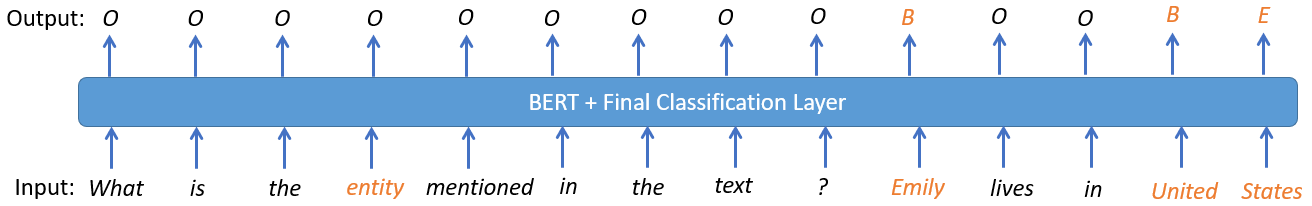
\includegraphics[width=\linewidth]{../thesis/span_detection}
    \caption{Span Detection Setup with \texttt{BIOE} scheme and \textit{What} as question word (colored tokens depict the generic entity type in question and gold entity mentions with expected output labels)}
    \label{fig:span_detection}
\end{figure}

